\documentclass{beamer}

\mode<presentation> {


%\usetheme{default}
%\usetheme{AnnArbor}
%\usetheme{Antibes} 
%\usetheme{Bergen}
%\usetheme{Berkeley}
%\usetheme{Berlin}
%\usetheme{Boadilla}
%\usetheme{CambridgeUS}
%\usetheme{Copenhagen}
%\usetheme{Darmstadt}
%\usetheme{Dresden}
%\usetheme{Frankfurt}
%\usetheme{Goettingen}
%\usetheme{Hannover}
%\usetheme{Ilmenau}
%\usetheme{JuanLesPins}
%\usetheme{Luebeck}
\usetheme{Madrid}
%\usetheme{Malmoe}
%\usetheme{Marburg}
%\usetheme{Montpellier}
%\usetheme{PaloAlto}
%\usetheme{Pittsburgh}
%\usetheme{Rochester}
%\usetheme{Singapore}
%\usetheme{Szeged}
%\usetheme{Warsaw}
%\usecolortheme{albatross}
%\usecolortheme{beaver}
%\usecolortheme{beetle}
%\usecolortheme{crane}
%\usecolortheme{dolphin}
%\usecolortheme{dove}
%\usecolortheme{fly}
%\usecolortheme{lily}
%\usecolortheme{orchid}
%\usecolortheme{rose}
%\usecolortheme{seagull}
%\usecolortheme{seahorse}
%\usecolortheme{whale}
%\usecolortheme{wolverine}

%\setbeamertemplate{footline} % To remove the footer line in all slides uncomment this line
%\setbeamertemplate{footline}[page number] % To replace the footer line in all slides with a simple slide count uncomment this line

%\setbeamertemplate{navigation symbols}{} % To remove the navigation symbols from the bottom of all slides uncomment this line
}

\usepackage{graphicx} % Allows including images
\graphicspath{{/Users/justindoty/Documents/Research/Structural_Estimation/ProductionHeterogeneity_in_Firms/R_Code/}}
\usepackage{booktabs} % Allows the use of \toprule, \midrule and \bottomrule in tables
\usepackage{amsmath}
\usepackage{amssymb}
\usepackage{mathrsfs}
\usepackage{caption}
\usepackage{subcaption}
\usepackage{bbm} 
\usepackage{xcolor}
%----------------------------------------------------------------------------------------
%	TITLE PAGE
%----------------------------------------------------------------------------------------

\title[Quantile Production Functions]{Heterogeneity in Firms:\\
A Proxy Variable Approach to Quantile Production Functions}

\author{Justin Doty and Suyong Song} % 
\institute[] % Your institution as it will appear on the bottom of every slide, may be shorthand to save space
{
\\  
\medskip % Your email address
}
\date{\today} % Date, can be changed to a custom date

\begin{document}

\begin{frame}
\titlepage % Print the title page as the first slide
\end{frame}

%----------------------------------------------------------------------------------------
%	PRESENTATION SLIDES
%----------------------------------------------------------------------------------------

%------------------------------------------------
\section{First Section} % Sections can be created in order to organize your presentation into discrete blocks, all sections and subsections are automatically printed in the table of contents as an overview of the talk
%------------------------------------------------

\subsection{Subsection Example} % A subsection can be created just before a set of slides with a common theme to further break down your presentation into chunks

\begin{frame}
\frametitle{Introduction}
\begin{itemize}
\item Identification issues: optimal input choices are functions of unobserved productivity leads to transmission bias
\pause
\item Popular control function approaches
\begin{itemize}
	\item OP (1994): Simultaneity and selection, investment policy proxy, application to telecommunications industry
	\item LP (2003): Intermediate input proxy, identification issues related to timing of labor input decisions, application to Chilean manufacturing firms
	\item ACF (2015): Value-Added production with intermediate input Proxy, identification under different DGPs, timing of labor matters
\end{itemize}
\pause
\item These approaches have focused on estimates of output elasticities on location of conditional firm-size distribution
\item Also, productivity heterogeneity are estimated average TFP measurements, typical dispersion measurements (e.g. 90-10 range) are average measurements.
\item There could be considerable heterogeneity not captured by average estimates

\end{itemize}
\end{frame}

%------------------------------------------------------------------------------------

\begin{frame}
\frametitle{Levinsohn and Petrin (2003)}
\begin{itemize}
	\item Brief review of LP approach
	\pause
	\item LP consider the following gross output production function (subscript $i$ omitted)
	\begin{equation}
	y_{t}=\beta_{0}+\beta_{k}k_{t}+\beta_{l}l_{t}+\beta_{\iota}\iota_{t}+\omega_{t}+\varepsilon_{t}
	\end{equation}
	\pause
	Where $\omega_{t}$ is productivity observed by the firm, but unobserved by the researcher (e.g, management quality, expected defect rates, etc.) and $\varepsilon_{t}$ represents iid shocks to production after making input choices at time $t$
	With the following assumptions
	\medskip
	\begin{enumerate}
		\pause
		\item Information Set: $\mathcal{I}_{t}$ includes current and past productivity shocks, but not future productivity. $\mathbb{E}[\varepsilon_{t}|\mathcal{I}_{t}]=0$
		\item First Order Markov: Productivity shocks evolve according to the distribution $p(\omega_{t}|\omega_{t-1})$
		\item Capital Accumulation: $k_{t}=\kappa(k_{t-1}, l_{t-1})$
		\item Scalar Unobservability: $\iota_{t}=\iota_{t}(k_{t}, \omega_{t})$
		\item Strict Monotonicity: $\iota_{t}=\iota_{t}(k_{t}, \omega_{t})$ is strictly increasing in $\omega_{t}$
	\end{enumerate}
\end{itemize}
\end{frame}

%------------------------------------------------------------------------------------

\begin{frame}
\frametitle{Levinsohn and Petrin (2003)}
\begin{itemize}
	\item Given these assumptions intermediate input demand can be inverted $\omega_{t}=\omega_{t}(k_{t}, \iota_{t})$ and substituted into the production function
	\begin{equation}
		y_{t}=\beta_{0}+\beta_{k}k_{t}+\beta_{l}l_{t}+\omega_{t}(k_{t}, \iota_{t})+\varepsilon_{t}=\beta_{l}l_{t}+\Phi(k_{t}, \iota_{t})+\varepsilon_{t}
	\end{equation}
	where $\Phi(k_{t}, \iota_{t})=\beta_{0}+\beta_{k}k_{t}+\beta_{\iota}\iota_{t}+\omega_{t}(k_{t}, \iota_{t})$
	\pause
	\item $\Phi(k_{t}, \iota_{t})$ can be estimated nonparametrically
	\item Labor coefficient and other variable coefficients are identified in the first stage
	\item First stage estimates are $\hat{\beta}_{l}$ and $\hat{\Phi}(k_{t}, \iota_{t})$ 
	\item Let $y^{*}=y-\hat{\beta}_{l}l_{t}$ denote the output net of labor contribution
\end{itemize}
\end{frame}

%------------------------------------------------------------------------------------

\begin{frame}
\frametitle{Levinsohn and Petrin (2003)}
\begin{itemize}
	\item Two moment conditions identify $\beta_{k}$ and $\beta_{\iota}$
	\item Capital does not respond to the innovation in productivity 
	\item Last period's input choice should not be correlated with the innovation in productivity this period
	\pause
	\begin{equation}
	\mathbb{E}[(\varepsilon_{t}+\eta_{t})Z_{t-1}]=\mathbb{E}[(y_{t}^{*}-\beta_{k}k_{t}-\beta_{\iota}\iota_{t}-\hat{\mathbb{E}}[\omega_{t}|\omega_{t-1}])Z_{t-1}]
	\end{equation}
	\pause
	\item $\hat{\mathbb{E}}[\omega_{t}|\omega_{t-1}]$ can be estimated using the estimates of $\omega_{t}$ from first stage estimates evaluated at $(\beta_{k}, \beta_{\iota})$
	\item $Z_{t-1}$ includes $k_{t}$ and $\iota_{t-1}$ as well as additional instruments
	\item LP minimize GMM criterion function and bootstrap standard errors 
\end{itemize}
\end{frame}


%------------------------------------------------------------------------------------

\begin{frame}
\frametitle{Heterogeneous Coefficient Models}
\begin{itemize}
	\item The control function approaches of OP, LP, and ACF estimate homogeneous output elasticities
	\item Many interesting questions can be asked if we consider production functions that are heterogeneous between firms
	\item Kasahara, Schrimpf and Suzuki (2015) propose two methods to estimate a random coefficient production function and find evidence of unobserved heterogeneity beyond a Hicks-neutral technology term
	\item Balat, Brambilla, and Sasaki (2015) extend the control function approach to infinitely supported coefficients with an application to international trade
	\item Li and Sasaki (2017) develop an identification strategy for heterogeneous elasticities using first order conditions for intermediate inputs
\end{itemize}
\end{frame}
%------------------------------------------------------------------------------------

\begin{frame}
\frametitle{Production Functions and Quantile Regression}
\begin{itemize}
	\item Allowing firm technology to vary over the conditional output distribution is also valid for estimating a production function with unobserved heterogeneity
	\item Applications of quantile regression are however limited due to simultaneity bias
	\item Typical IV approaches such as Chernozhukov and Hansen (2005) are also limited due to availability of instruments (input prices) and arguing for the monotonicity of the unobserved heterogeneity
	\item Possible to exploit the panel data structure and use fixed effects (Koenker, 2004), Lamarche (2010), or Canay (2011)
	\item The fixed effect shifts the location of the conditional distribution (not the quantiles)
	\item Incidental Parameters (Koenker, 2004)
	\item Independence of unobserved heterogeneity and productivity (Canay, 2011)
	
\end{itemize}
\end{frame}


%------------------------------------------------------------------------------------

\begin{frame}
\frametitle{Quantile Production Function}
We seek to extend the control function approach to a quantile value-production function for a fixed $\tau\in(0,1]$ defined as
\begin{equation}
	Q_{\tau}(y_{t}|k_{t}, l_{t})=\beta_{k}(\tau)k_{t}+\beta_{l}(\tau)l_{t}+\omega_{t}
\end{equation}
\pause
\begin{itemize}
	\item $l_{t}$ is a freely variable input like labor and $k_{t}$ denotes the state variable as capital input
	\item $\omega_{t}$ is an unobserved state variable to the econometrician that impacts firm's optimal input decisions
	\item We allow for inputs to affect quantiles of the output distribution
	\item A special case of this quantile production function is the location scale model
	\pause
	\begin{equation}
	 y_{it}=\beta_{k}k_{it}+\beta_{l}l_{it}+\omega_{it}+(\eta_{k}k_{it}+\eta_{l}l_{it}+\eta_{\omega}\omega_{it})\varepsilon_{it}
	\end{equation}
	\pause
	which implies that the $\tau$-th conditional quantile of $y_{it}$ is given by
	\begin{equation}
	Q_{\tau}(y_{it}|\mathcal{I}_{it})=\beta_{k}k_{it}+\beta_{l}l_{it}+\omega_{it}+(\eta_{k}k_{it}+\eta_{l}l_{it}+\eta_{\omega}\omega_{it})F^{-1}(\tau)
	\end{equation}
\end{itemize}
\end{frame}
%------------------------------------------------------------------------------------

\begin{frame}
\frametitle{Quantile Production Function: Assumptions}
We maintain several timing assumptions that are standard in the control function literature\\

We use the set of assumptions for LP estimation, but can be easily altered for ACF as we do both in simulations\\
\pause

\begin{enumerate}
	\item Information Set: $\mathcal{I}_{t}$ includes current and past productivity shocks, but not future productivity. $Q_{\tau}(\varepsilon_{t}|\mathcal{I}_{t})=0$
	\item Firm's productivity follows an AR(1) process
	\begin{equation}
		\omega_{t}=\mathbb{E}[\omega_{t}|\omega_{t-1}]+\xi_{t}=g(\omega_{t-1})+\xi_{t}
	\end{equation}
	\item Capital Accumulation: $k_{t}=\kappa(k_{t-1}, i_{t-1})$
	\item Scalar Unobservability: $\iota_{t}=\iota_{t}(k_{t}, \omega_{t};\tau)$
	\item Strict Monotonicity: $\iota_{t}=\iota_{t}(k_{t}, \omega_{t};\tau)$ is strictly increasing in $\omega_{t}$
\end{enumerate}
\end{frame}

%------------------------------------------------------------------------------------

\begin{frame}
\frametitle{Quantile Production Function: Estimation}
\begin{itemize}
	\item Given these assumptions we invert intermediate input demand $\omega_{t}=\omega_{t}(k_{t}, \iota_{t})$ and substitute into the production function
	\begin{equation}
	Q_{\tau}(y_{t}|k_{t}, l_{t})=\beta_{l}(\tau)l_{t}+\beta_{k}(\tau)k_{t}+\omega_{t}(k_{t}, \iota_{t})=\beta_{l}(\tau)l_{t}+\Phi(k_{t}, \iota_{t})
	\end{equation}
	\pause
	\item First stage parameters $\beta_{l}(\tau)$ and $\Phi(k_{t}, \iota_{t})$ are estimated here
	\item If one uses a polynomial approximation to $\Phi(k_{t}, \iota_{t})$, $\hat{\beta}_{l}(\tau)$ and $\hat{\Phi}(k_{t}, \iota_{t})$ can be estimated using a polynomial quantile regression
	\pause
	\item Substituting into the production
	\begin{equation}
	Q_{\tau}(y_{t}|k_{t}, l_{t})=\beta_{k}(\tau)k_{t}+\hat{\beta}_{l}(\tau)l_{t}+g(\hat{\Phi}(k_{t-1}, \iota_{t-1})-\beta_{k}(\tau)k_{t-1})+\xi_{t}
	\end{equation}
	\pause
	\item This equation is complicated by the unobservable $\xi_{t}$, we will assume that its sum with the production function shock $\varepsilon_{t}$ is conditional quantile zero, but this may not be valid
\end{itemize}
\end{frame}

%------------------------------------------------------------------------------------

\begin{frame}
\frametitle{Quantile Production Function: Estimation}
We can write a second stage conditional quantile restriction as
\small
\begin{equation}
Q_{\tau}[y_{t}-\beta_{k}(\tau)k_{t}-\hat{\beta}_{l}(\tau)l_{t}-g(\hat{\Phi}_{\tau}(k_{t-1}, \iota_{t-1})-\beta_{k}(\tau)k_{t-1})|\mathcal{I}_{it-1}]=0
\end{equation}
\normalsize
\pause
\begin{itemize}
	\item The model in (10) can be represented by conditional moment restrictions
	\small
	\begin{equation}
	\mathbb{E}[\mathbbm{1}\{y_{t}-\beta_{k}(\tau)k_{t}-\hat{\beta}_{l}(\tau)l_{t}-g(\hat{\Phi}_{\tau}(k_{t-1}, \iota_{t-1})-\beta_{k}(\tau)k_{t-1})\leq 0\}-\tau|\mathcal{I}_{it-1}]=0
	\end{equation}
	\normalsize
	where $\mathbbm{1}\{\cdot\}$ is the indicator function
	\pause
	\item To estimate the production function parameters we use the unconditional moments
	\small
	\begin{equation}
	\mathbb{E}[Z_{t-1}(\mathbbm{1}\{y_{t}-\beta_{k}(\tau)k_{t}-\hat{\beta}_{l}(\tau)l_{t}-g(\hat{\Phi}_{\tau}(k_{t-1}, \iota_{t-1})-\beta_{k}(\tau)k_{t-1})\leq 0\}-\tau)]=0
	\end{equation}
	\normalsize
	where $Z_{t-1}$ includes the instruments used in the firm's information set at time $t-1$
\end{itemize}
	
\end{frame}
%------------------------------------------------------------------------------------

\begin{frame}
\frametitle{Smoothed GMM for Quantile Models}
\begin{itemize}
	\item The indicator function makes estimation of the production function parameters intractable
	\item We smooth the indicator function and rely on the theory and estimation procedure of de Castro, Galvao, Kaplan and Liu (2018)
	\item Develops theory for feasible estimators of parameters in general conditional quantile restrictions that include non-linear IVQR
	\item This approach is computationally attractive compared to approaches such as the MCMC approach proposed by Chernozhukov and Hong (2003)
	\pause
	\item To fix notation let
	\begin{itemize}
		\item $Z_{t-1}$ the set of instruments discussed earlier
		\item $x_{t}$ the set of exogenous and endogenous covariates
		\item $\Lambda(\cdot)$ denote the residual function that defines the conditional quantile restriction that is known up to $\beta_{k}(\tau)$
	\end{itemize}
	
\end{itemize}
\end{frame}
%------------------------------------------------------------------------------------

\begin{frame}
\frametitle{Smoothed GMM for Quantile Models}
\begin{itemize}
	\item The sample analog of (12) can be written as:
	\begin{equation}
    \hat{M}_{n}(\beta, \tau)=\frac{1}{NT}\sum_{i=1}^{N}\sum_{t=1}^{T}Z_{it}\Bigg[\tilde{I}\Bigg(\frac{\Lambda(y_{it}, x_{it}, \beta(\tau))}{h_{n}}\Bigg)-\tau\Bigg],
	\end{equation}
	\pause
	where $h_{n}$ is a bandwidth (sequence) and $\tilde{I}(\cdot)$ is a smoothed version of the indicator function $\mathbbm{1}\{\cdot \leq 0\}$ used by Horowitz (1998), Whang (2006), and Kaplan and Sun (2016):
	\begin{equation}
	    \tilde{I}(u)=\mathbbm{1}\{-1\leq u \leq 1\}\big[0.5+\frac{105}{64}\big(u-\frac{5}{3}u^{3}+\frac{7}{5}u^{5}- \frac{3}{7}u^{7}\big)\big]+\mathbbm{1}\{u>1\}.
	\end{equation}
	\pause
	The smoothed GMM estimator minimizes a weighted quadratic norm of the smoothed sample moment vector
	\begin{equation}
		\hat{\beta}_{GMM}=\underset{\beta}{\operatorname{argmin}}\hat{M}_{n}(\beta, \tau)^{\top}\hat{W}\hat{M}_{n}(\beta, \tau).
		\end{equation}
\end{itemize}
\end{frame}

%------------------------------------------------------------------------------------

\begin{frame}
\frametitle{Smoothed GMM for Quantile Models}
\begin{itemize}
	\item The optimal weighting matrix is the estimator of the inverse long-run variance of the sample moment $\hat{W}^{*}=\bar{\Omega}^{-1}\overset{p}{\to}\Omega^{-1}$
	\item In simulation and in application we use the long-run variance estimator as in Newey and West (1987) with a truncated kernel. We find this helps with scaling the moment conditions
	\item The asymptotic results for this estimator cannot be applied here due to the semi-parametric nature of the two-step procedure
	\item We are working to see if the asymptotic results of Ai and Chen (2007) can be applied here. This gives us extra conditions to show what rate gives an asymptotically negligible bandwidth. The smoothed sample moments are differentiable so we can take a Taylor expansion around $\beta(\tau)$, but the bandwidth problem remains
	\item We use bootstrap for our empirical application
\end{itemize}
\end{frame}

%------------------------------------------------------------------------------------

\begin{frame}
\frametitle{Quantile Production Function: Simulation}
\begin{itemize}
	\item Simulations follow a location-scale version of LP (2003) and ACF (2015) using ACF's original set of DGPs 
	\item Parameters are chosen to match a couple of key moments in the Chilean data used by LP
	\item Productivity follows a first order AR(1) process with persistence $\rho=0.7$
	\item Firms make optimal choices of investment in the capital stock to maximize the expected discounted value of future profits
	\item Convex capital adjustment costs
	\item Labor input $l_{t}$ is chosen either at $t$ or $t-b$
	\item Possible optimization error in labor input decision
\end{itemize}
\end{frame}

%------------------------------------------------------------------------------------

\begin{frame}
\frametitle{Quantile Production Function: Simulation}
\begin{itemize}
	\item Production function is assumed Leontief in materials, the location-scale specification is
	\begin{equation}
		y_{t}=\beta_{k}k_{t}+\beta_{l}l_{t}+\omega_{t}+(0.7k_{t}+0.6l_{t}+0.1\omega_{t})\varepsilon_{t}
	\end{equation}
	with $\beta_{k}=0.4$, $\beta_{l}=0.6$\\
	\pause
	Simulation 1: ACF Estimated Quantile Production Function
	\begin{itemize}
		\item Firms face different wages, where the wage process following an AR(1) process
		\item Assume labor is chosen at time $t-b$ where $b=0.5$
	\end{itemize}
	\pause
	Simulation 2: LP Estimation Quantile Production Function
	\begin{itemize}
		\item No wage variation across firms and labor chosen at time $t$
		\item Added optimization error in labor
	\end{itemize}
	\pause
	\item Both simulations include 2 DGP's for the error term $\varepsilon_{t}$. In DGP 1 $\varepsilon_{t} \sim N(0,0.1)$ and in DGP 2 $\varepsilon_{t} \sim \textit{Laplace}(0,0.1)$
\end{itemize}
\end{frame}

%----------------------------------------------------------------------------------

\begin{frame}
\frametitle{Quantile Production Function: Simulation 1}
\begin{table}[ht]
\caption{Simulated precision of estimators of $\beta_{k}(\tau)$ and $\beta_{l}(\tau)$}
\centering
\resizebox{\linewidth}{!}{
\begin{tabular}{cccccccccc}
  \hline\hline & & \multicolumn{4}{c}{QACF} & \multicolumn{4}{c}{ACF} \\ \cmidrule(lr){3-6} \cmidrule(lr){7-10} \\& & \multicolumn{2}{c}{$\beta_{k}$}  & \multicolumn{2}{c}{$\beta_{l}$} &\multicolumn{2}{c}{$\beta_{k}$} & \multicolumn{2}{c}{$\beta_{l}$}  \\ \cmidrule(lr){3-4} \cmidrule(lr){5-6} \cmidrule(lr){7-8} \cmidrule(lr){9-10}DGP & $\tau$ & Bias & MSE & Bias & MSE & Bias & MSE & Bias & MSE \\ 
  \hline
1 & 0.10 & 0.0223 & 0.0007 & 0.0311 & 0.0016 & -0.0917 & 0.0089 & -0.0759 & 0.0060 \\ 
   & 0.25 & 0.0128 & 0.0003 & 0.0155 & 0.0005 & -0.0492 & 0.0029 & -0.0395 & 0.0018 \\ 
   & 0.50 & 0.0020 & 0.0001 & 0.0020 & 0.0002 & -0.0020 & 0.0005 & 0.0010 & 0.0002 \\ 
   & 0.75 & -0.0108 & 0.0003 & -0.0055 & 0.0003 & 0.0452 & 0.0025 & 0.0415 & 0.0019 \\ 
   & 0.90 & -0.1123 & 0.0146 & 0.0859 & 0.0095 & 0.0877 & 0.0082 & 0.0779 & 0.0063 \\ 
  2 & 0.10 & 0.0193 & 0.0014 & 0.0164 & 0.0024 & -0.1127 & 0.0135 & -0.0966 & 0.0098 \\ 
   & 0.25 & 0.0015 & 0.0005 & 0.0524 & 0.0044 & -0.0485 & 0.0032 & -0.0416 & 0.0022 \\ 
   & 0.50 & 0.0020 & 0.0001 & 0.0010 & 0.0002 & 0.0000 & 0.0008 & 0.0000 & 0.0005 \\ 
   & 0.75 & -0.0525 & 0.0056 & 0.0316 & 0.0044 & 0.0485 & 0.0032 & 0.0416 & 0.0022 \\ 
   & 0.90 & -0.0653 & 0.0080 & 0.0446 & 0.0059 & 0.1127 & 0.0135 & 0.0966 & 0.0098 \\ 
   \hline
\end{tabular}}
\caption*{1000 replications. Under location-scale, $\beta_{x}(\tau)=\beta_{x}+\eta_{x}F^{-1}(\tau)$ where $x=\{k,l\}, \eta_{x}=\{0.7, 0.6\}$ and $F$ is the CDF of $\varepsilon_{it}$}
\end{table}
\end{frame}

%----------------------------------------------------------------------------------

\begin{frame}
\frametitle{Quantile Production Function: Simulation 1}
\begin{figure}[H]
\centering
\caption{Simulated precision of estimators of $\beta_{k}(\tau)$ and $\beta_{l}(\tau)$. Dotted line is ACF estimator}
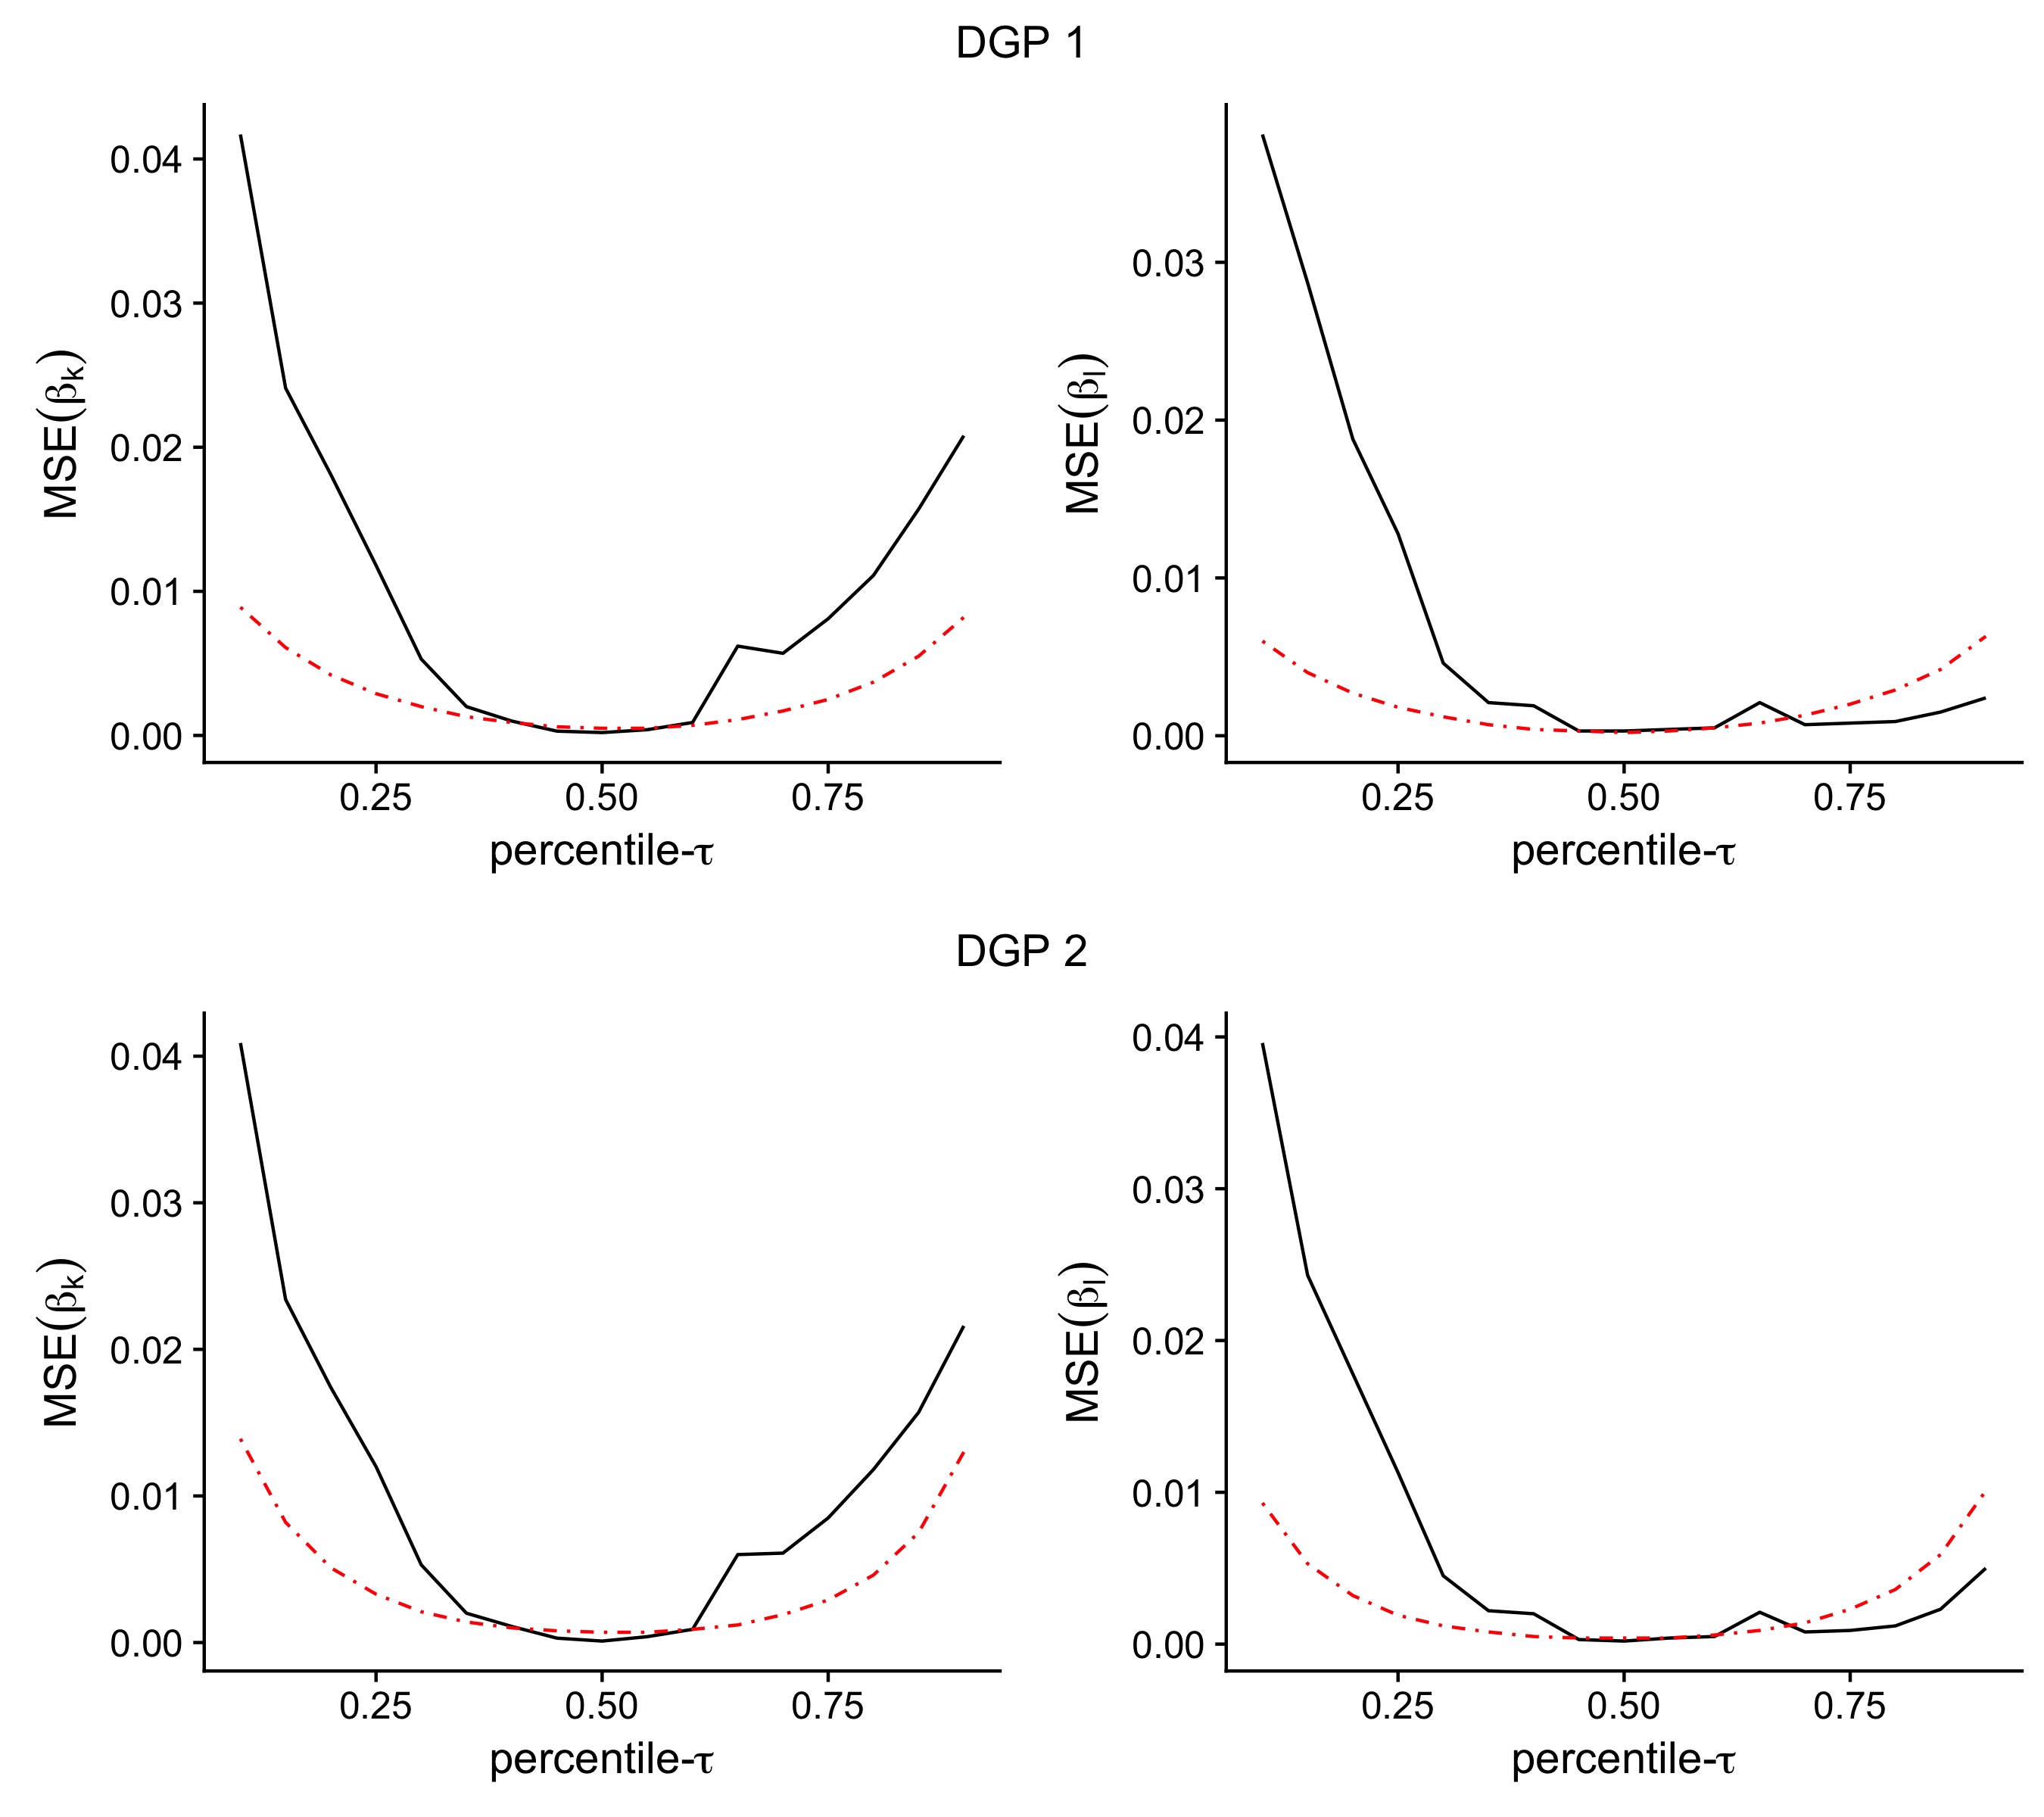
\includegraphics[width=12cm, height=6cm, keepaspectratio]{ACF_MSE_Plot.png}
\end{figure}
\end{frame}

%----------------------------------------------------------------------------------

\begin{frame}
\frametitle{Quantile Production Function: Simulation 2}
\begin{table}[ht]
\caption{Simulated precision of estimators of $\beta_{k}(\tau)$ and $\beta_{l}(\tau)$}
\centering
\resizebox{\linewidth}{!}{
\begin{tabular}{cccccccccc}
  \hline\hline & & \multicolumn{4}{c}{QLP} & \multicolumn{4}{c}{ACF} \\ \cmidrule(lr){3-6} \cmidrule(lr){7-10} \\& & \multicolumn{2}{c}{$\beta_{k}$}  & \multicolumn{2}{c}{$\beta_{l}$} &\multicolumn{2}{c}{$\beta_{k}$} & \multicolumn{2}{c}{$\beta_{l}$}  \\ \cmidrule(lr){3-4} \cmidrule(lr){5-6} \cmidrule(lr){7-8} \cmidrule(lr){9-10}DGP & $\tau$ & Bias & MSE & Bias & MSE & Bias & MSE & Bias & MSE \\ 
  \hline
1 & 0.10 & 0.0323 & 0.0027 & -0.0009 & 0.0012 & -0.0887 & 0.0088 & -0.0769 & 0.0063 \\ 
   & 0.25 & 0.0178 & 0.0013 & -0.0005 & 0.0007 & -0.0462 & 0.0031 & -0.0405 & 0.0020 \\ 
   & 0.50 & 0.0060 & 0.0011 & 0.0000 & 0.0006 & 0.0010 & 0.0010 & 0.0000 & 0.0004 \\ 
   & 0.75 & -0.0058 & 0.0006 & -0.0005 & 0.0008 & 0.0482 & 0.0033 & 0.0405 & 0.0020 \\ 
   & 0.90 & -0.0163 & 0.0013 & -0.0001 & 0.0011 & 0.0907 & 0.0092 & 0.0769 & 0.0063 \\ 
  2 & 0.10 & 0.0303 & 0.0036 & -0.0016 & 0.0036 & -0.1107 & 0.0141 & -0.0976 & 0.0104 \\ 
   & 0.25 & 0.0255 & 0.0020 & 0.0004 & 0.0013 & -0.0465 & 0.0040 & -0.0426 & 0.0027 \\ 
   & 0.50 & 0.0040 & 0.0003 & 0.0000 & 0.0004 & 0.0020 & 0.0018 & -0.0010 & 0.0009 \\ 
   & 0.75 & -0.0105 & 0.0014 & -0.0014 & 0.0014 & 0.0505 & 0.0044 & 0.0406 & 0.0025 \\ 
   & 0.90 & -0.0113 & 0.0039 & -0.0034 & 0.0039 & 0.1147 & 0.0150 & 0.0956 & 0.0100 \\ 
   \hline
\end{tabular}}
\caption*{1000 replications. Under location-scale, $\beta_{x}(\tau)=\beta_{x}+\eta_{x}F^{-1}(\tau)$ where $x=\{k,l\}, \eta_{x}=\{0.7, 0.6\}$ and $F$ is the CDF of $\varepsilon_{it}$}
\end{table}
\end{frame}

%----------------------------------------------------------------------------------

\begin{frame}
\frametitle{Quantile Production Function: Simulation 2}
\begin{figure}[H]
\centering
\caption{Simulated precision of estimators of $\beta_{k}(\tau)$ and $\beta_{l}(\tau)$. Dotted line is LP estimator}
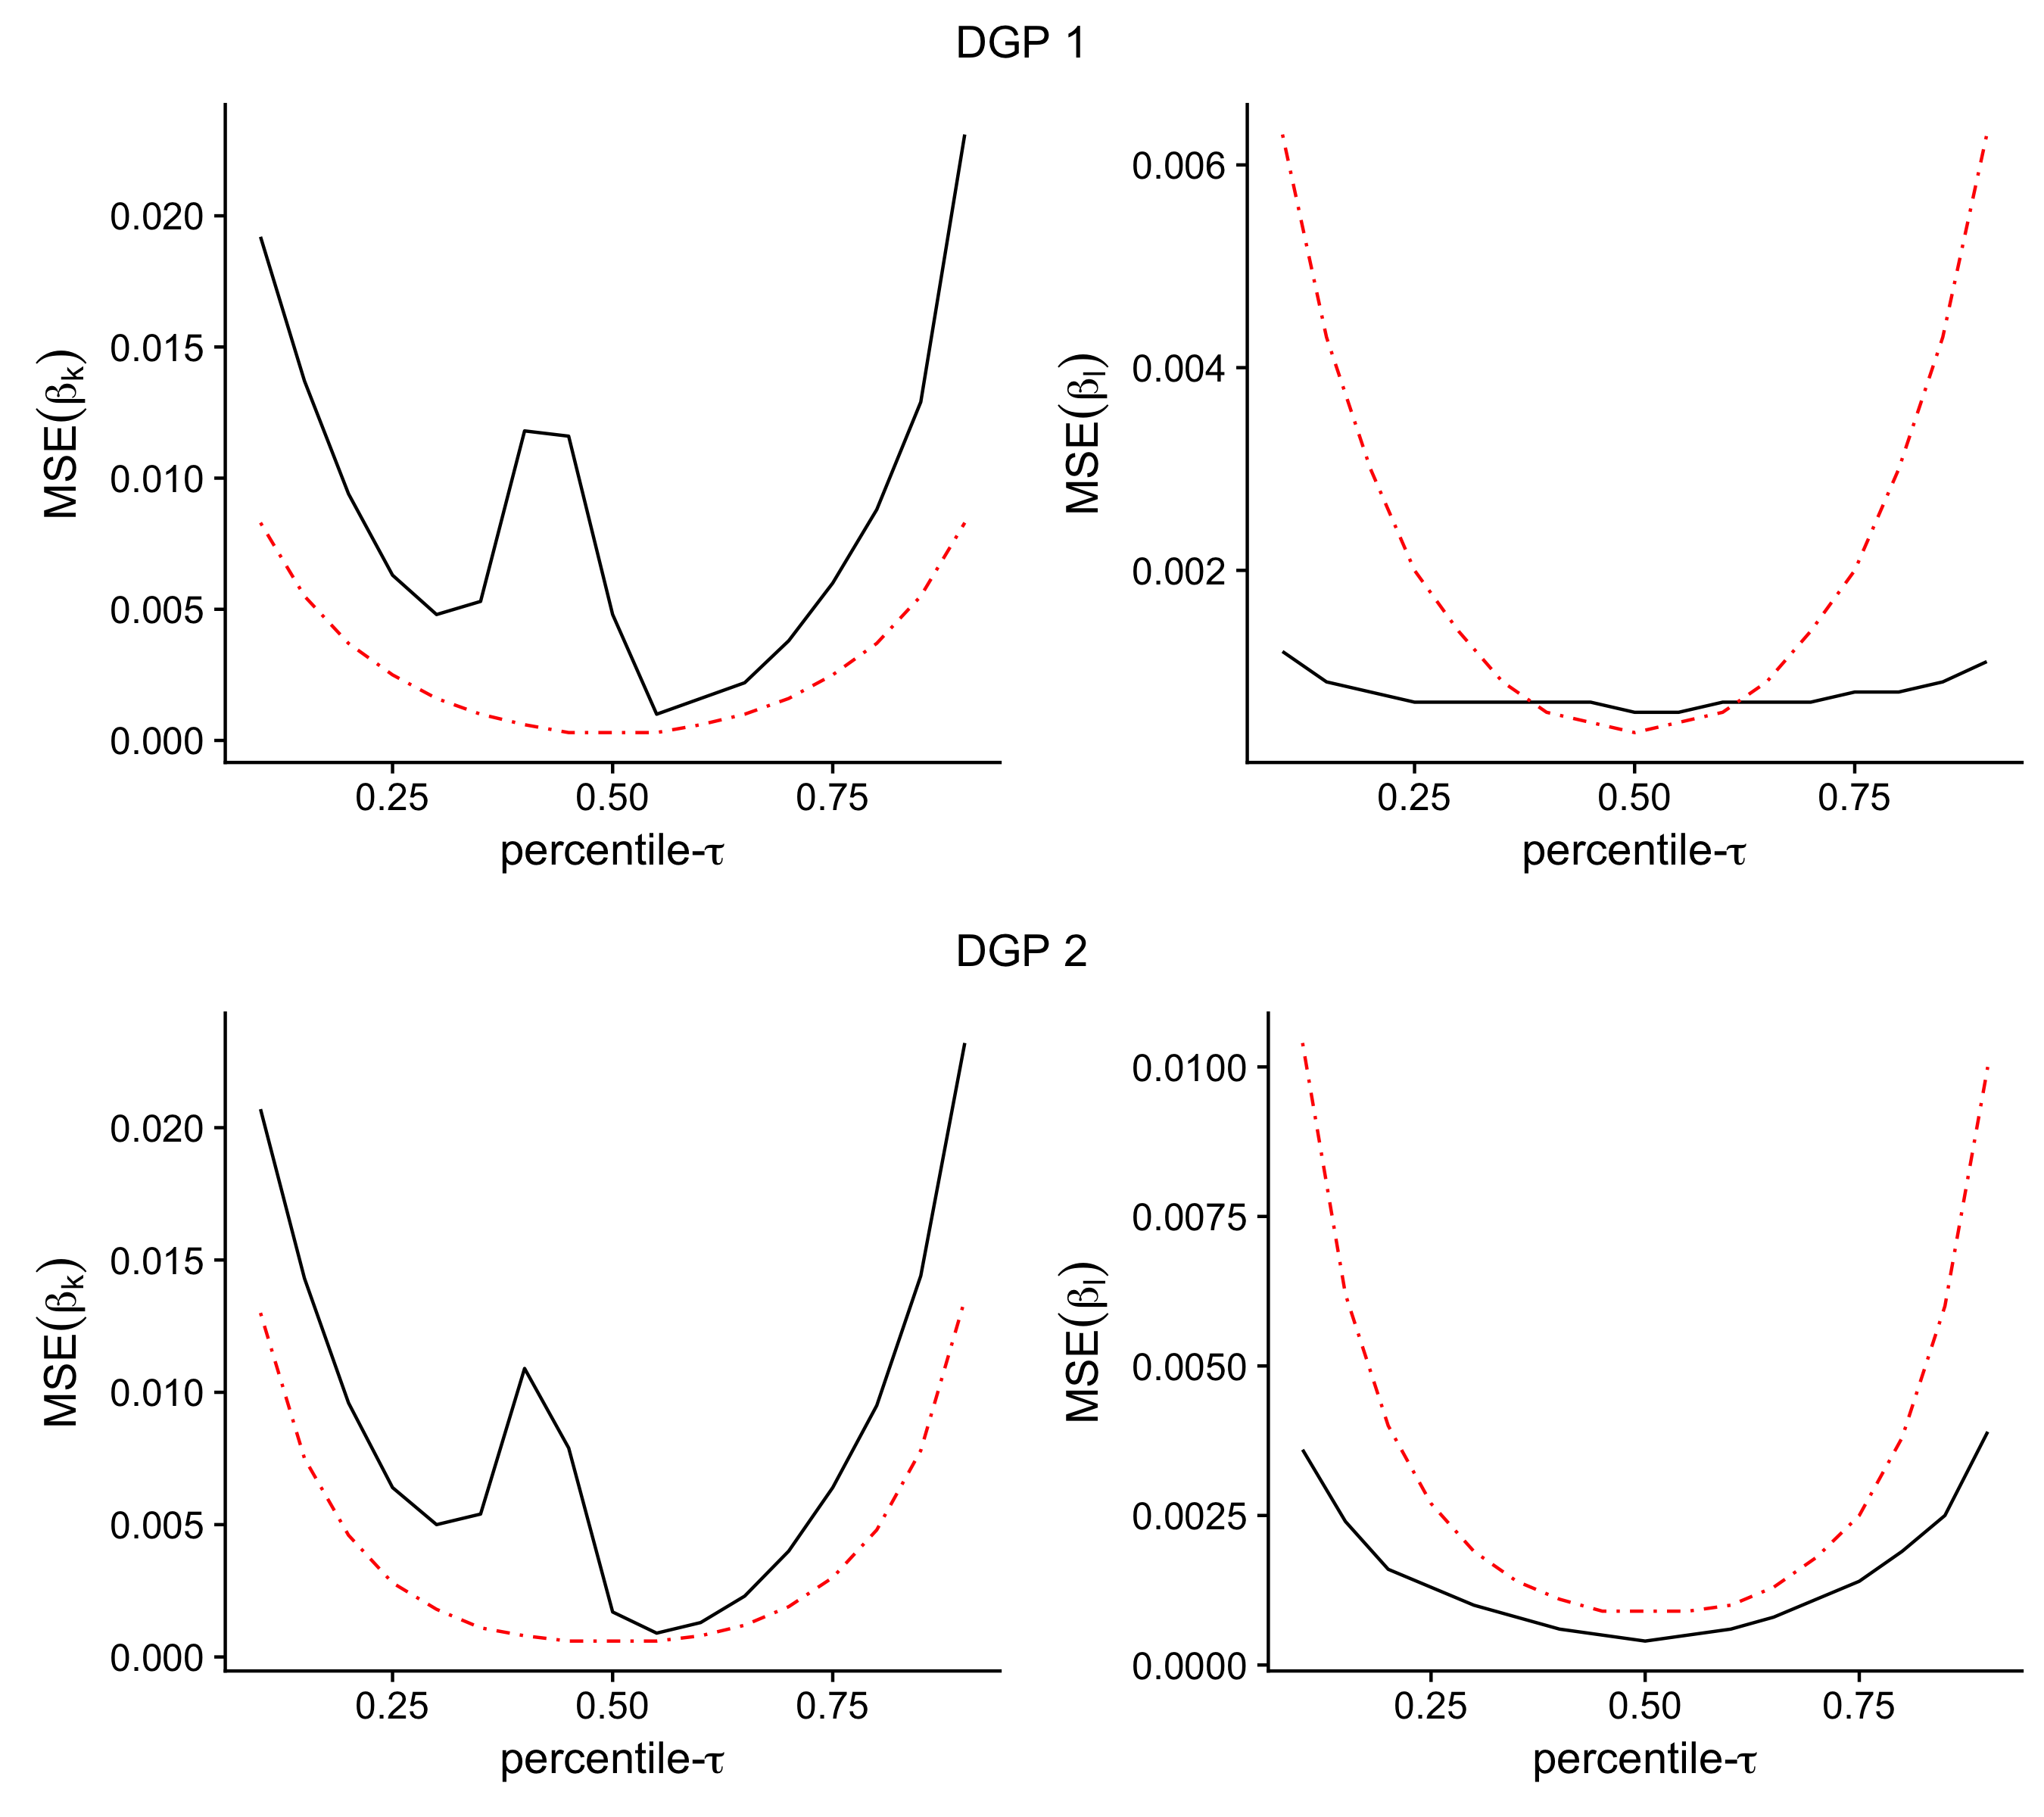
\includegraphics[width=12cm, height=6cm, keepaspectratio]{LP_MSE_Plot.png}
\end{figure}
\end{frame}

%----------------------------------------------------------------------------------


\begin{frame}
\frametitle{Quantile Production Function: Application}
\begin{itemize}
	\item We apply this estimator to an 10-year panel (1987-1996) from Chile (ENIA) provided by Amil Petrin 
	\item Focus on the four largest industries (ISIC codes in parentheses): Food Products (311), Metals (381), Textiles (321) and Wood Products (331)
	\item We use the QLP estimator for a value-added specification of the production function
	\item Standard errors are obtained from the bootstrapping method outlined by Levinsohn and Petrin (2003)
	\item Comparison to LP approach is provided and implemented by prodest.R package (Gabrielle Rovigatti)
\end{itemize}
\end{frame}

%----------------------------------------------------------------------------------

\begin{frame}
\frametitle{Quantile Production Function: Simulation 2}
\begin{table}[ht]
\caption{Parameter estimates for four industries (bootstrapped standard errors)}
\centering
\resizebox{\linewidth}{!}{
\begin{tabular}{cccccccccc}
  \hline\hline & & \multicolumn{2}{c}{Capital}  & \multicolumn{2}{c}{Skilled Labor} & \multicolumn{2}{c}{Unskilled Labor} & \multicolumn{2}{c}{Returns to Scale} \\ \cmidrule(lr){3-4} \cmidrule(lr){5-6} \cmidrule(lr){7-8} \cmidrule(lr){9-10}Industry (ISIC code) & $\tau$ & Coef. & s.e. & Coef. & s.e. & Coef. & s.e. & Coef. & s.e \\ 
  \hline
311 & 0.10 & 0.278 & 0.0570 & 0.313 & 0.0402 & 0.516 & 0.0443 & \textcolor{red}{1.107} & 0.0793 \\ 
   & 0.25 & 0.126 & 0.0375 & 0.274 & 0.0249 & 0.464 & 0.0298 & 0.865 & 0.0490 \\ 
   & 0.50 & 0.235 & 0.0444 & 0.246 & 0.0187 & 0.429 & 0.0241 & \textcolor{red}{0.909} & 0.0522 \\ 
   & 0.75 & 0.235 & 0.0561 & 0.209 & 0.0206 & 0.417 & 0.0263 & 0.861 & 0.0652 \\ 
  381 & 0.10 & \textcolor{red}{0.166} & 0.1123 & 0.465 & 0.0846 & 0.596 & 0.0772 & \textcolor{red}{1.228} & 0.1188 \\ 
   & 0.25 & 0.371 & 0.0981 & 0.393 & 0.0534 & 0.524 & 0.0675 & 1.288 & 0.1063 \\ 
   & 0.50 & 0.244 & 0.0783 & 0.399 & 0.0401 & 0.417 & 0.0469 & \textcolor{red}{1.061} & 0.0838 \\ 
   & 0.75 & 0.218 & 0.0622 & 0.367 & 0.0347 & 0.396 & 0.0305 & \textcolor{red}{0.981} & 0.0707 \\ 
  321 & 0.10 & 0.262 & 0.1278 & 0.545 & 0.0585 & 0.476 & 0.0692 & 1.283 & 0.1351 \\ 
   & 0.25 & 0.160 & 0.1144 & 0.511 & 0.0521 & 0.385 & 0.0558 & \textcolor{red}{1.056}& 0.1126 \\ 
   & 0.50 & 0.171 & 0.0665 & 0.492 & 0.0495 & 0.386 & 0.0545 & \textcolor{red}{1.049} & 0.0778 \\ 
   & 0.75 & 0.227 & 0.0613 & 0.442 & 0.0524 & 0.392 & 0.0627 & \textcolor{red}{1.061} & 0.0744 \\ 
  331 & 0.10 & 0.208 & 0.1020 & 0.435 & 0.0522 & 0.583 & 0.0728 & \textcolor{red}{1.225} & 0.1271 \\ 
   & 0.25 & 0.144 & 0.0662 & 0.378 & 0.0610 & 0.481 & 0.0676 & \textcolor{red}{1.003} & 0.0942 \\ 
   & 0.50 & 0.176 & 0.0580 & 0.351 & 0.0396 & 0.431 & 0.0498 & \textcolor{red}{0.959} & 0.0742 \\ 
   & 0.75 & 0.127 & 0.0600 & 0.378 & 0.0365 & 0.314 & 0.0410 & 0.819 & 0.0683 \\ 
   \hline
\end{tabular}}
\end{table}
\end{frame}

%----------------------------------------------------------------------------------

\begin{frame}
\frametitle{Quantile Production Function: Application}
\begin{figure}[H]
\centering
\caption{Estimated values of production function coefficients and their 90\% confidence interval}
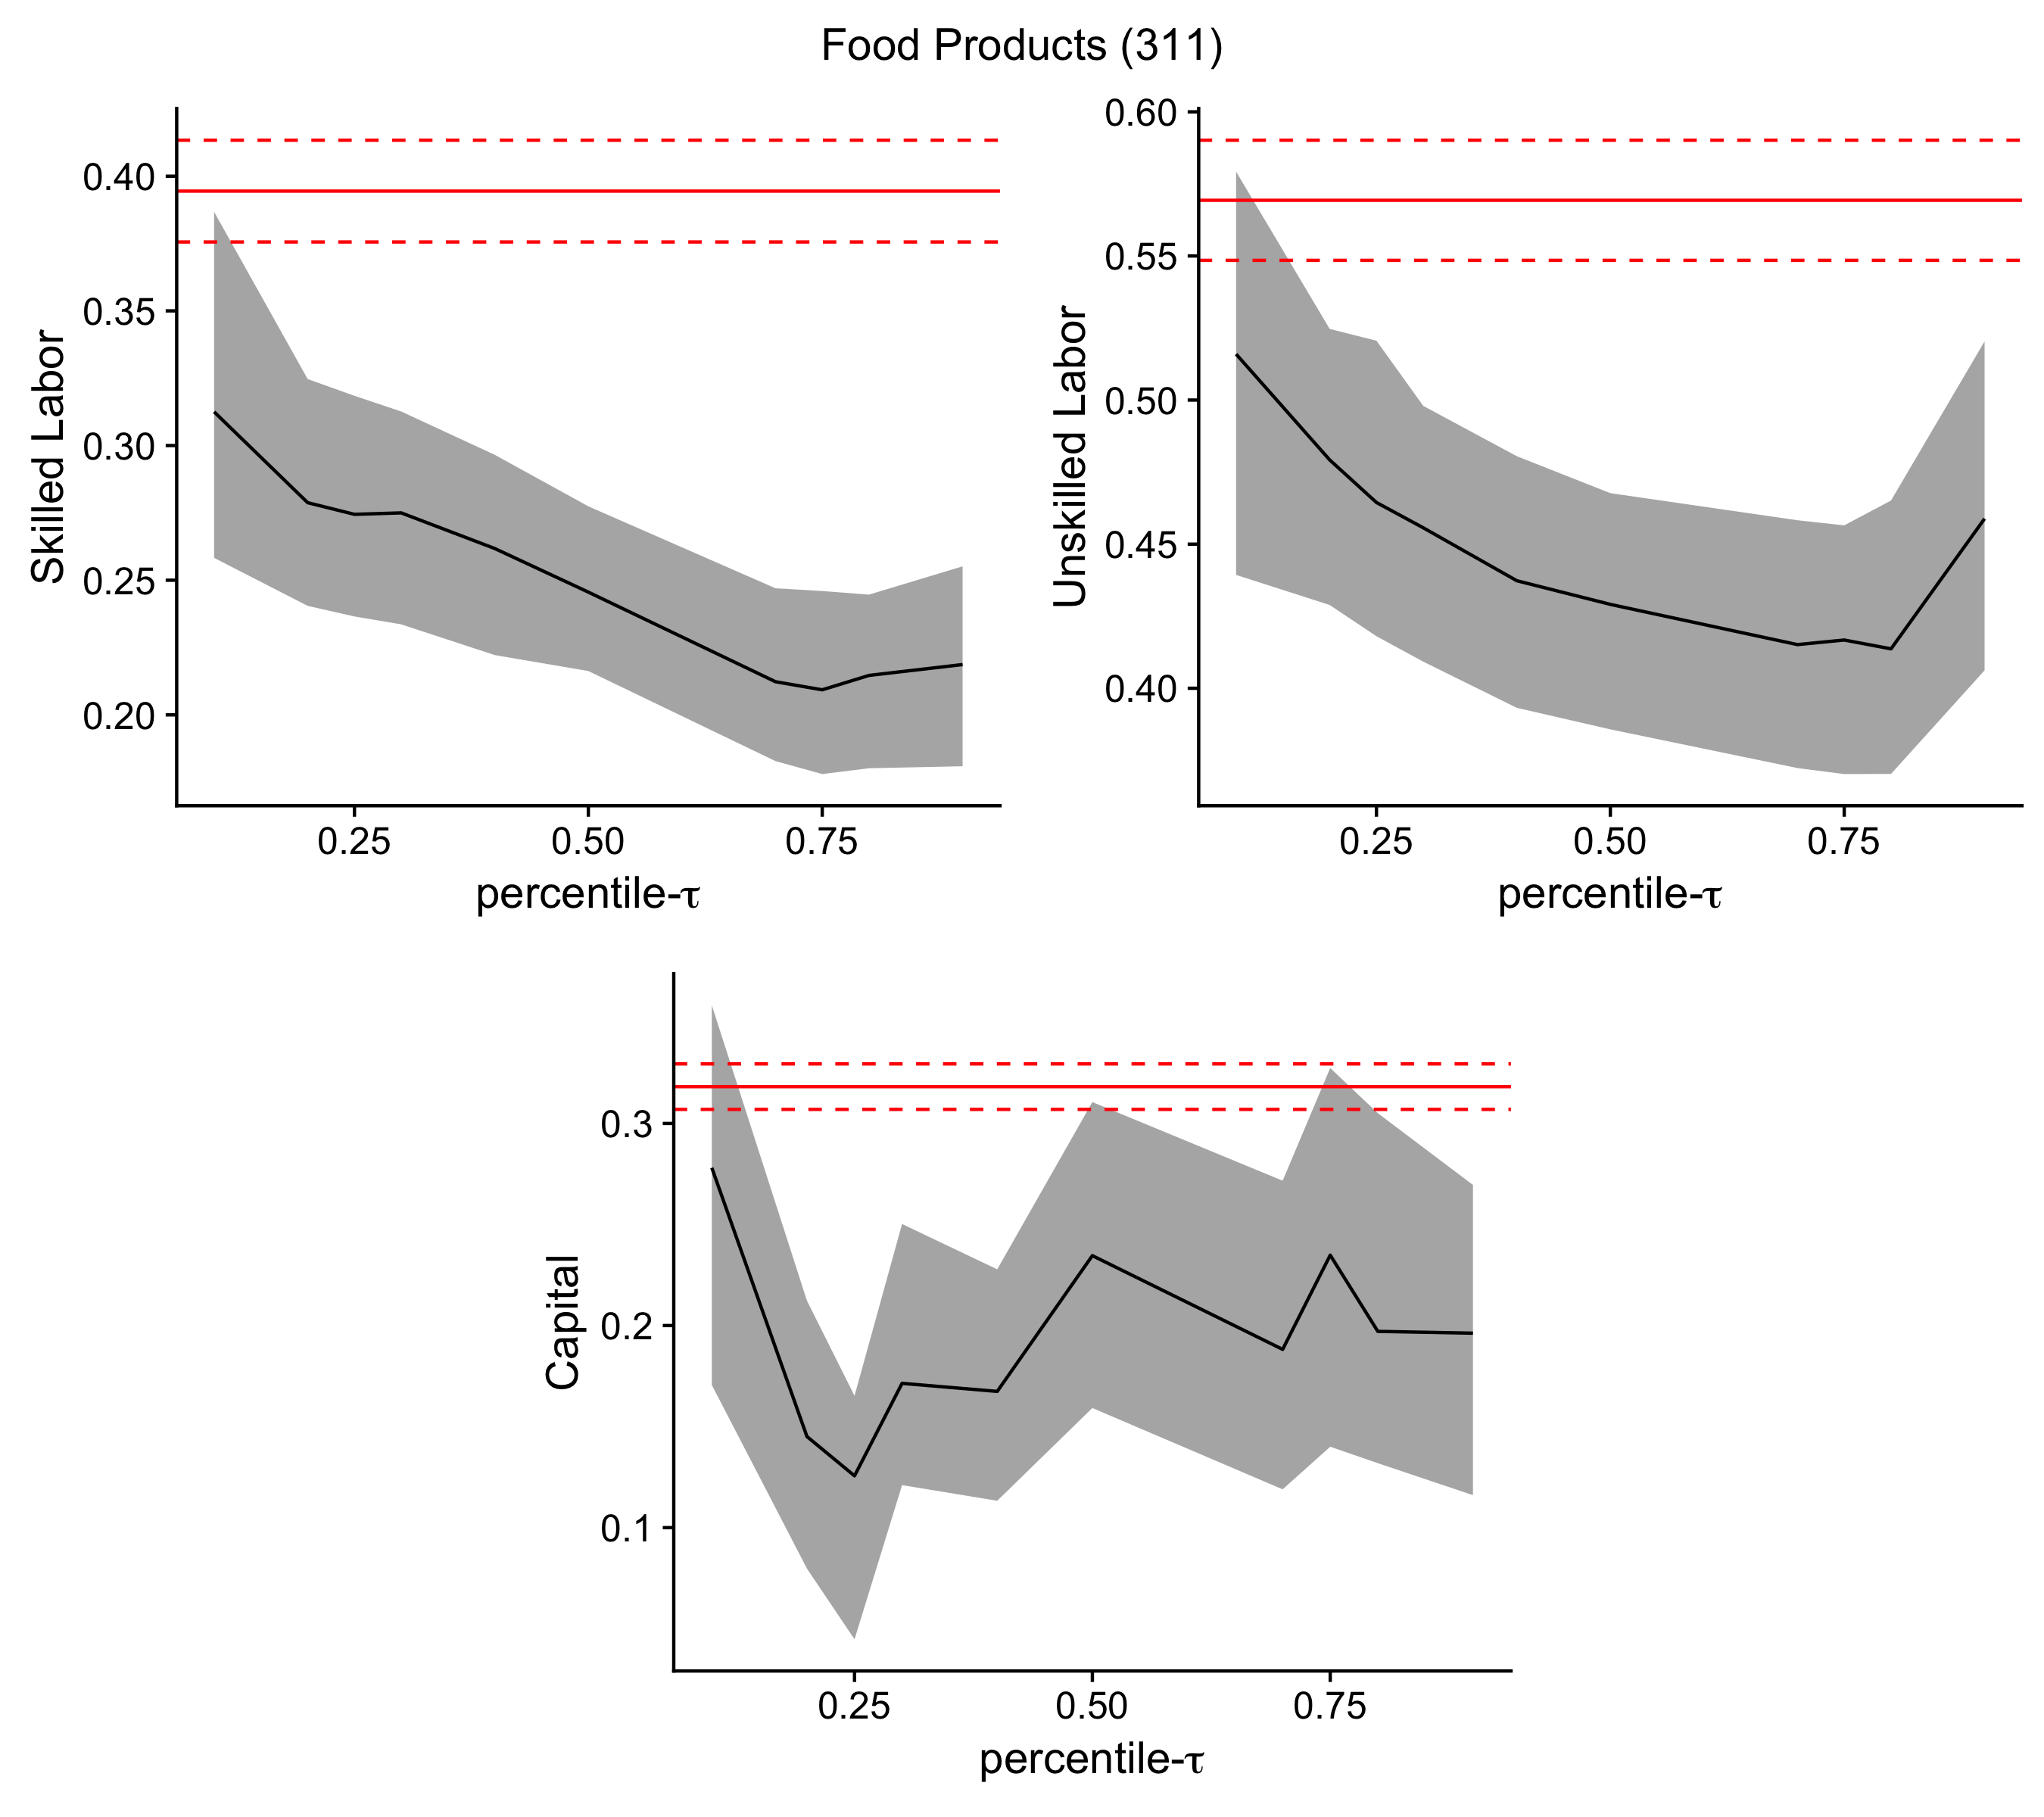
\includegraphics[width=12cm, height=6cm, keepaspectratio]{Coefficient_Plot_1.png}
\end{figure}
\end{frame}

%----------------------------------------------------------------------------------

\begin{frame}
\frametitle{Quantile Production Function: Application}
\begin{figure}[H]
\centering
\caption{Estimated values of production function coefficients and their 90\% confidence interval}
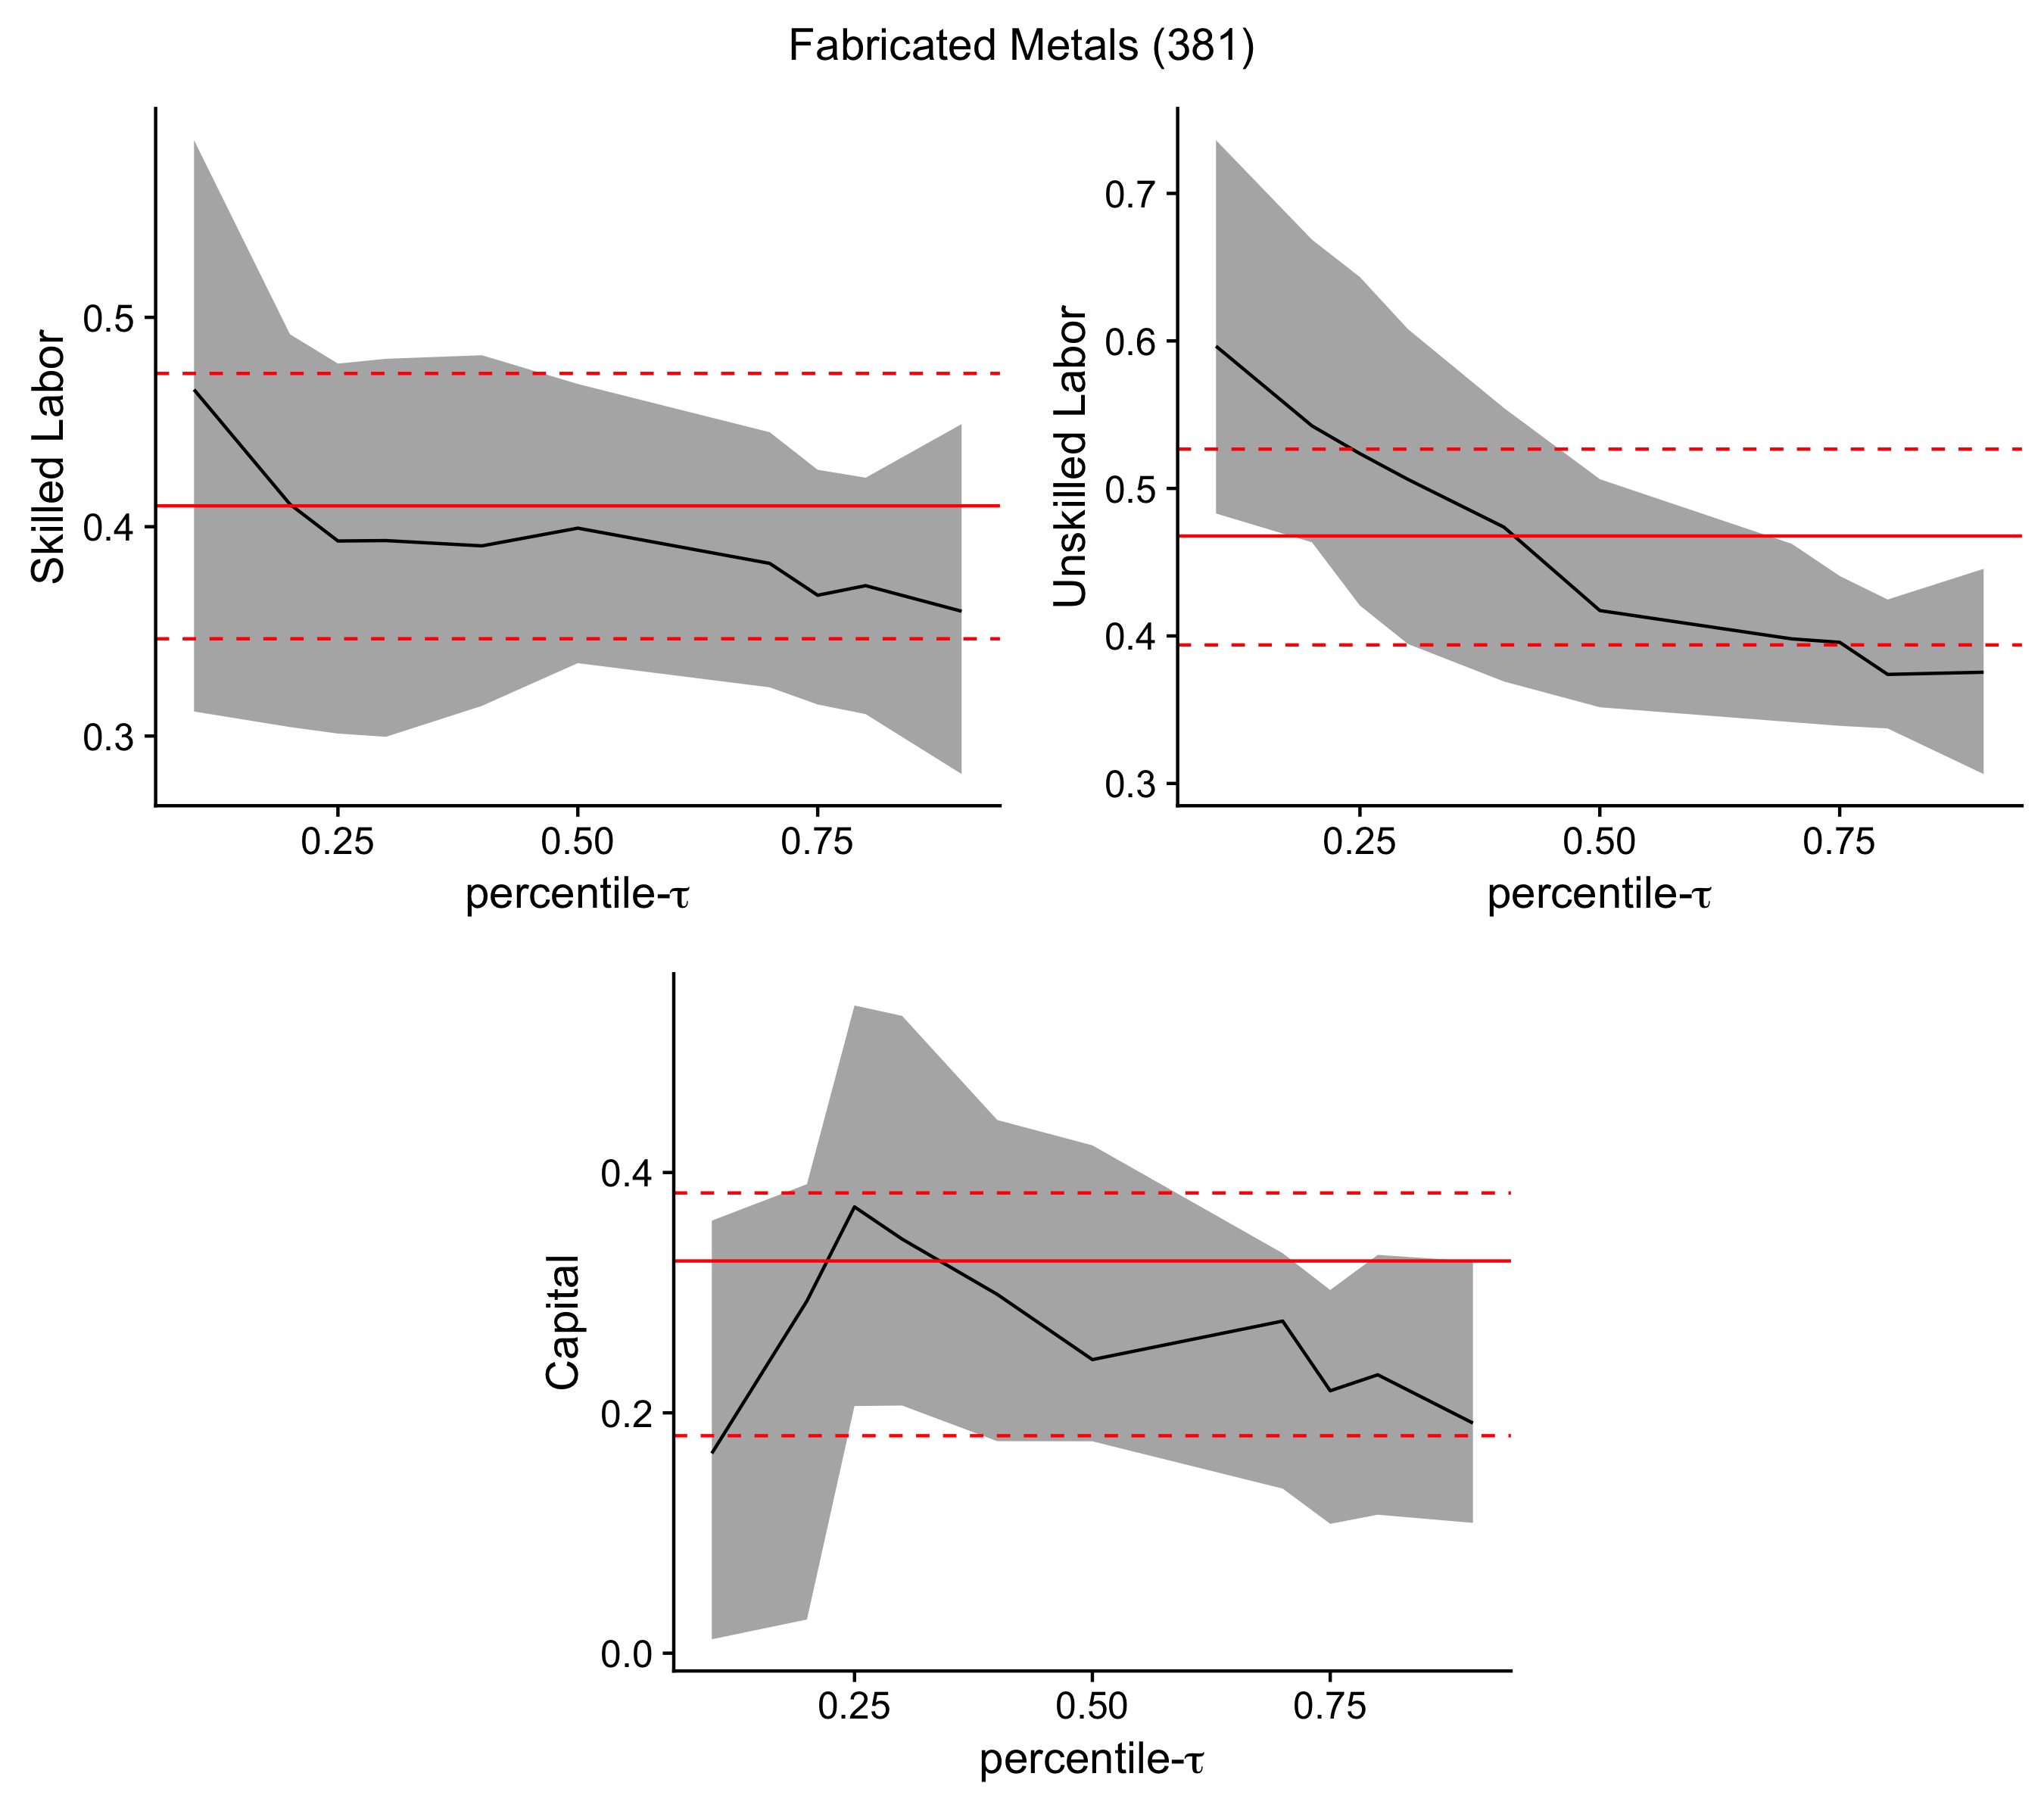
\includegraphics[width=12cm, height=6cm, keepaspectratio]{Coefficient_Plot_2.png}
\end{figure}
\end{frame}

%----------------------------------------------------------------------------------

\begin{frame}
\frametitle{Quantile Production Function: Application}
\begin{figure}[H]
\centering
\caption{Estimated values of production function coefficients and their 90\% confidence interval}
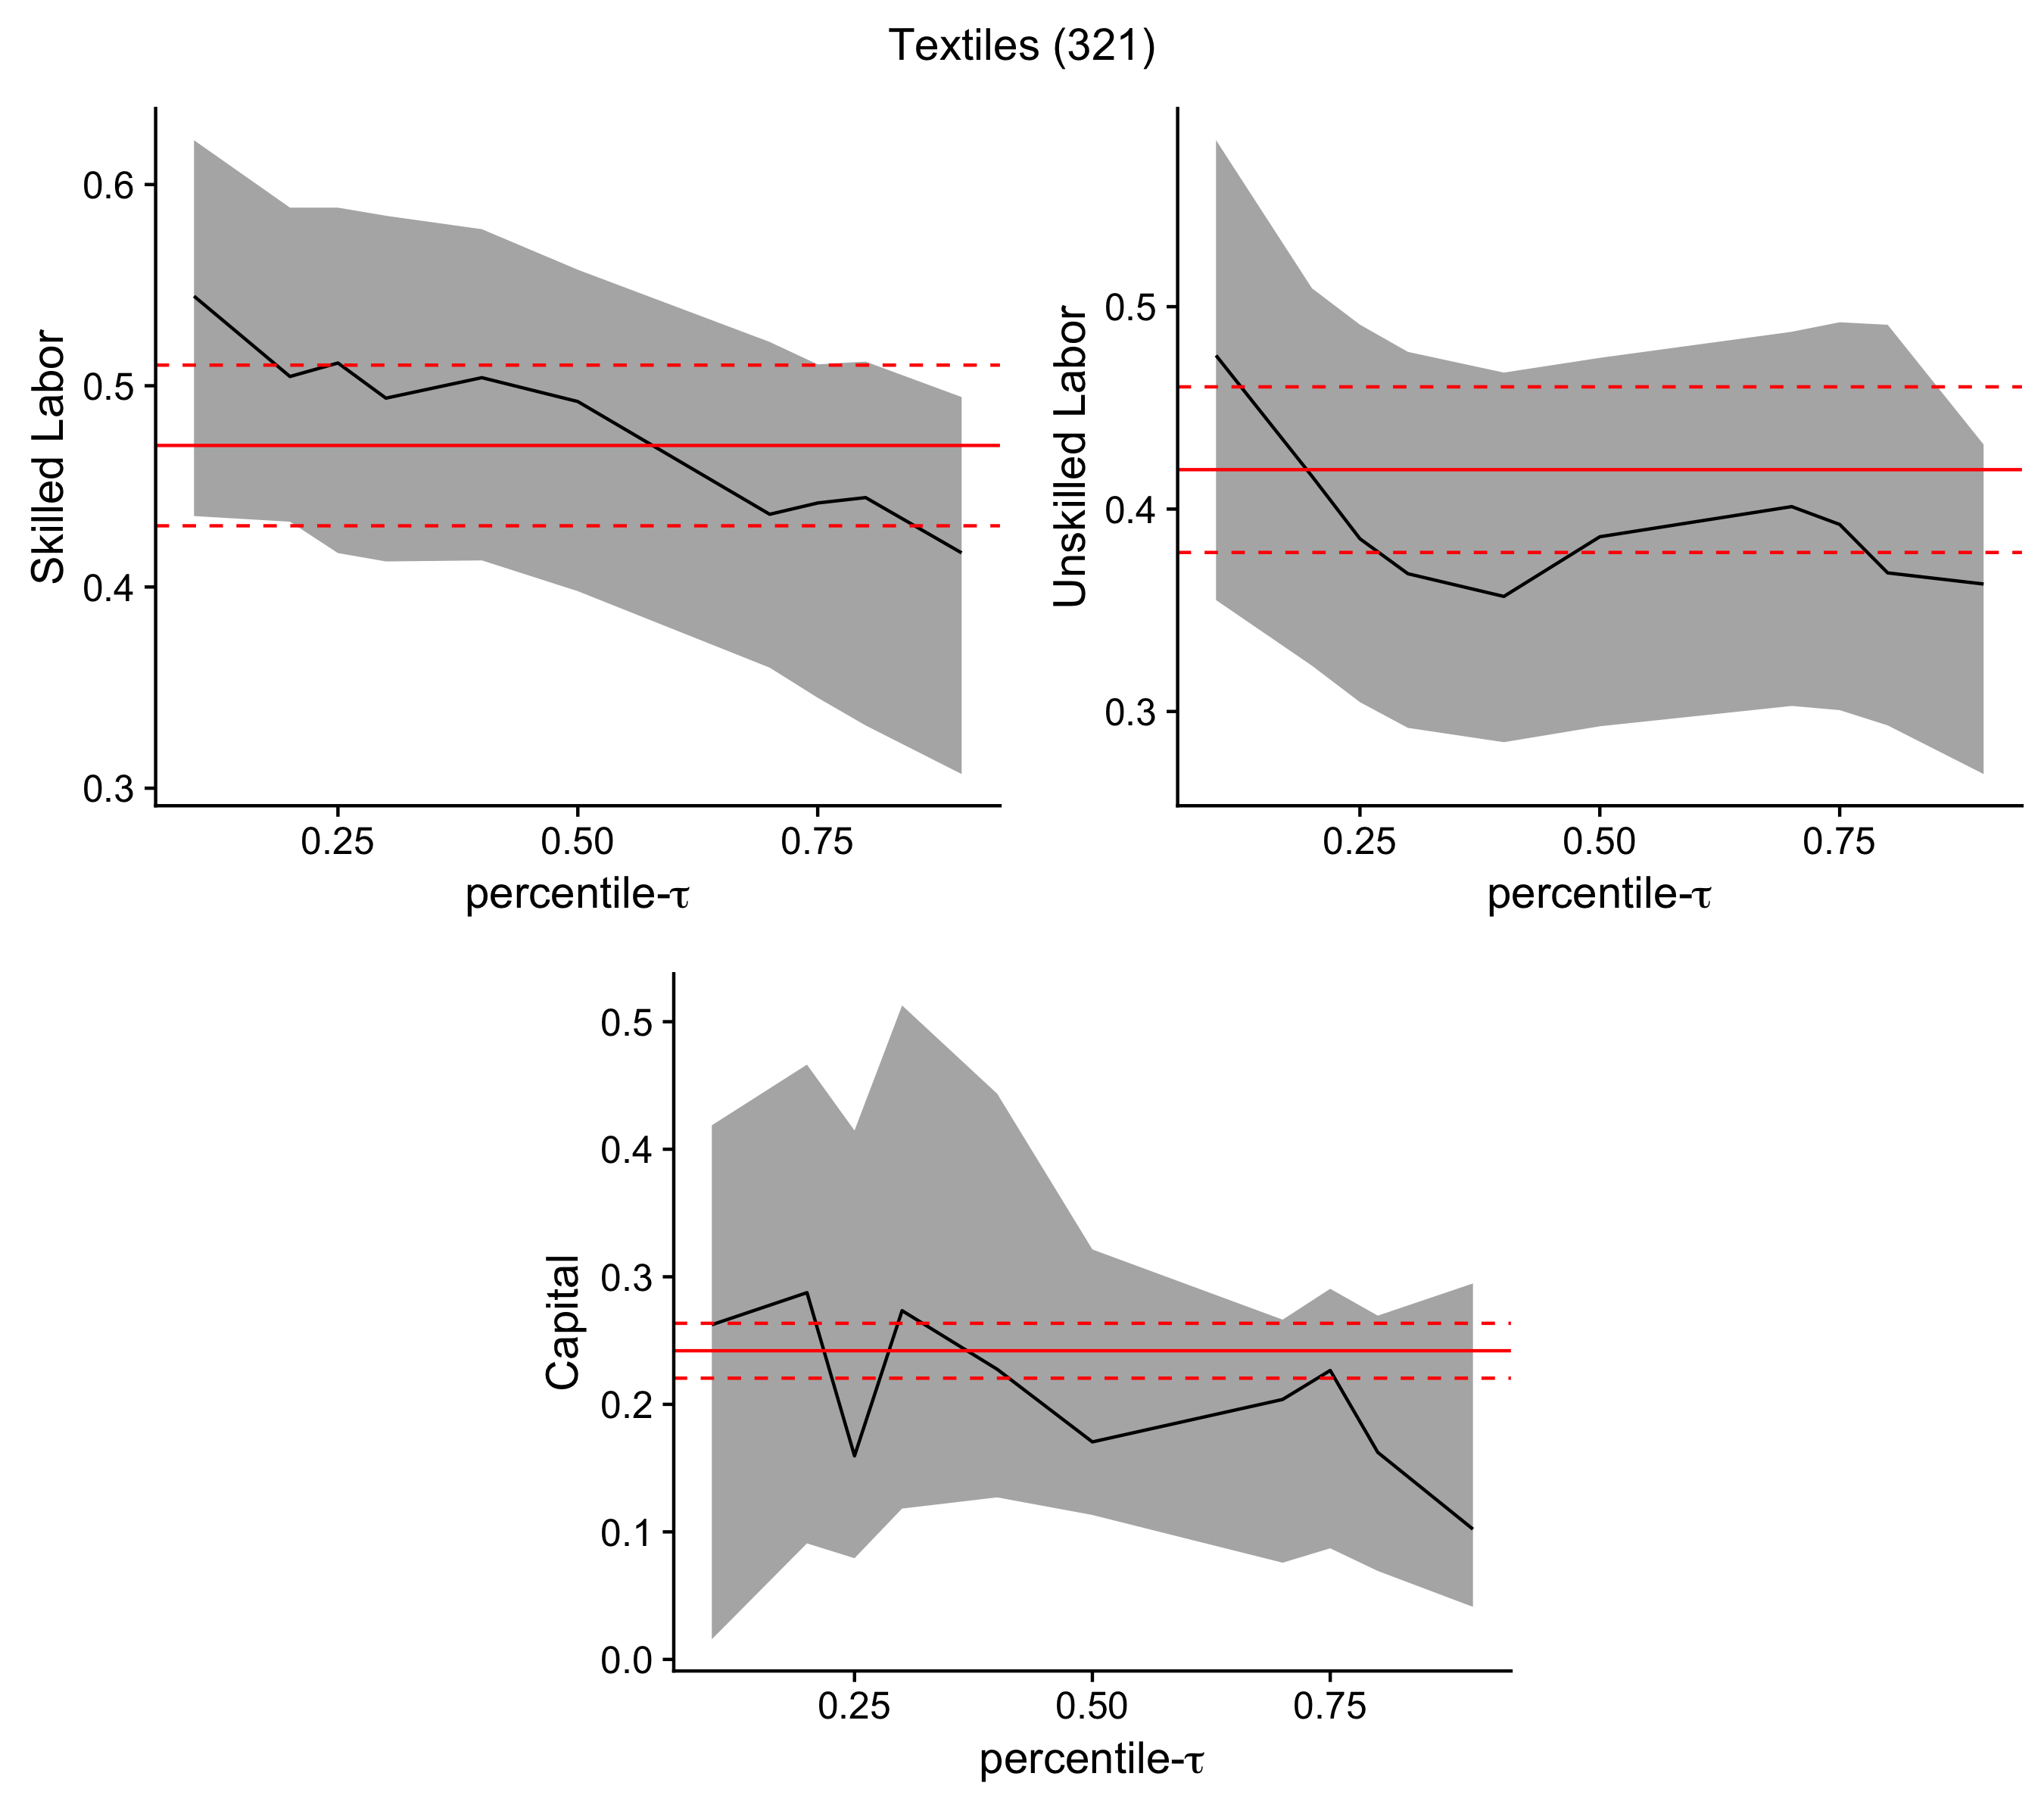
\includegraphics[width=12cm, height=6cm, keepaspectratio]{Coefficient_Plot_3.png}
\end{figure}
\end{frame}

%----------------------------------------------------------------------------------

\begin{frame}
\frametitle{Quantile Production Function: Application}
\begin{figure}[H]
\centering
\caption{Estimated values of production function coefficients and their 90\% confidence interval}
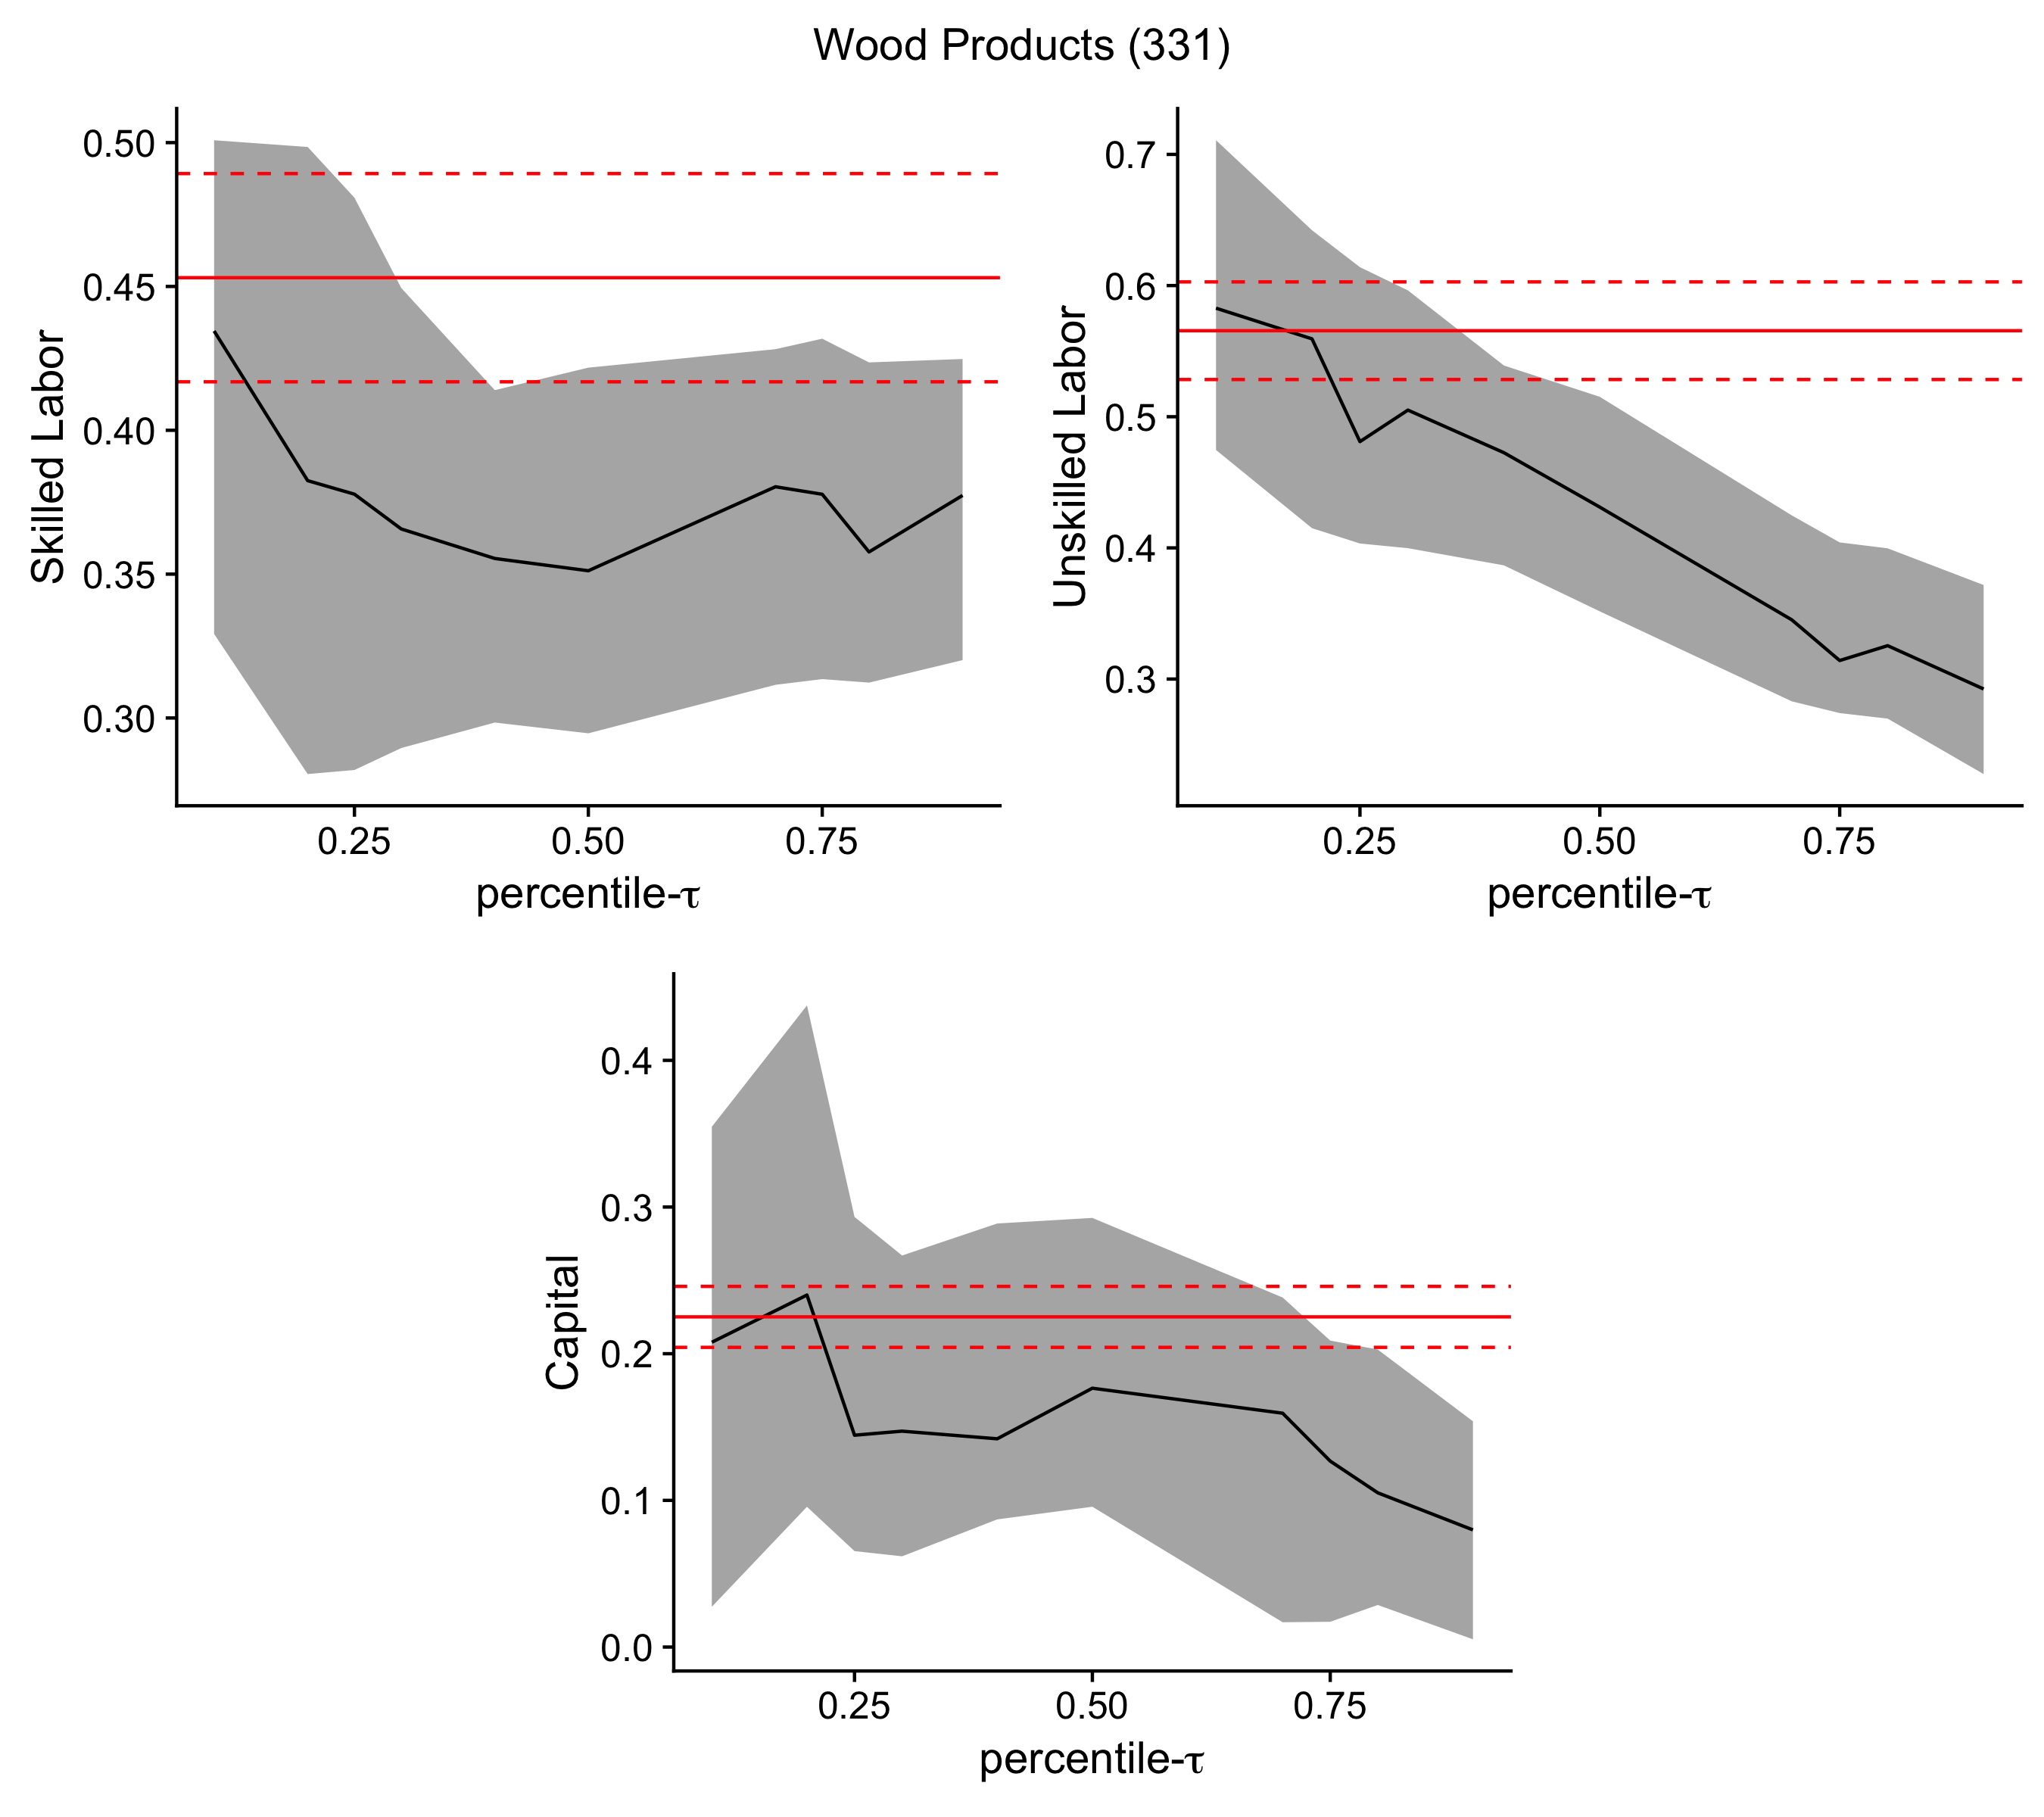
\includegraphics[width=12cm, height=6cm, keepaspectratio]{Coefficient_Plot_4.png}
\end{figure}
\end{frame}

%----------------------------------------------------------------------------------

\begin{frame}
\frametitle{Quantile Production Function: Conclusion}
\begin{itemize}
	\item While these quantile estimates exhibit interesting trends, they are not statistically different from the mean estimates
	\item Perhaps a different data application would be better
	\item Still working on asymptotic results and a numerically feasible implementation such as Ackerberg, Chen, Hahn, and Liao (2014)
	\item Implications for TFP measurements, a new way to look at TFP dispersion
	\item Working on implementing additional tests: Wald test for constant effects across quantiles, over-identification tests and an alternative model specification
\end{itemize}
\end{frame}

%----------------------------------------------------------------------------------

\begin{frame}
\frametitle{Alternative Estimator: Integrated Moment Condition}
We have the following moment condition from earlier (now including $\xi$ ($i,t$ omitted))
\begin{equation}
	\mathbb{E}[Z(\mathbbm{1}\{y-\beta_{k}(\tau)k-\hat{\beta}_{l}(\tau)l-g(\hat{\Phi}_{\tau}(k, \iota)-\beta_{k}(\tau)k)-\xi\leq 0\}-\tau)]=0
	\end{equation}
	or 
\begin{equation}
	\mathbb{E}[Z(\mathbbm{1}\{y-\beta_{k}(\tau)k-\hat{\beta}_{l}(\tau)l-g(\hat{\Phi}_{\tau}(k, \iota)-\beta_{k}(\tau)k)\leq \xi\}-\tau)]=0
\end{equation}
Assume $\xi \sim N(\beta_{0}(\tau),\sigma^{2})$. Applying law of iterated expectations we obtain the following integrated moment condition
\small
\begin{equation}
	\mathbb{E}[\frac{1}{\sqrt{2\pi}\sigma}\int_{-\infty}^{\infty}Z(\mathbbm{1}\{y-\beta_{k}(\tau)k-\hat{\beta}_{l}(\tau)-g(\hat{\Phi}_{\tau}(k, \iota)-\beta_{k}(\tau)k)\leq \xi\}-\tau)e^{\frac{-\xi}{2\sigma^{2}}}]=0
\end{equation}
Need to consider the case when $\xi\geq0$ and $\xi<0$ inside the indicator function. For example, consider when $\xi\geq0$
\end{frame}

%----------------------------------------------------------------------------------

\begin{frame}
\frametitle{Alternative Estimator: Integrated Moment Condition}
The integral of the indicator function when $\xi\geq 0$
\begin{equation}
	\frac{1}{\sqrt{2\pi}\sigma}\int_{-\infty}^{\infty}\mathbbm{1}\{y-\beta_{k}(\tau)k-\hat{\beta}_{l}(\tau)l-g(\hat{\Phi}_{\tau}(k, \iota)-\beta_{k}(\tau)k)\leq \xi\}
\end{equation}
Is equal to (with simplification)
\begin{equation}
	1-\Psi\Big(\frac{\Lambda(y, x, \beta(\tau))-\beta_{0}(\tau)}{\sigma}\Big)
\end{equation}
Similarly when $\xi<0$ we obtain
\begin{equation}
	\Psi\Big(\frac{\Lambda(y, x, \beta(\tau))-\beta_{0}(\tau)}{\sigma}\Big)
\end{equation}
where $\Lambda(y, x, \beta(\tau))$ is the residual function defined earlier (without $\xi$) and $\Psi(\cdot)$ is the CDF of standard normal
\end{frame}

%----------------------------------------------------------------------------------

\begin{frame}
\frametitle{Alternative Estimator: Integrated Moment Condition}
The integrated moment function becomes
\begin{equation}
\begin{split}
	\mathbb{E}\Bigg[Z\Bigg(&\mathbbm{1}\{\Lambda(y, x, \beta(\tau))\geq0\}\Bigg(1-\Psi\Big(\frac{\Lambda(y, x, \beta(\tau))-\beta_{0}(\tau)}{\sigma}\Big)\Bigg)+
	\\&\mathbbm{1}\{\Lambda(y, x, \beta(\tau))<0\}\Bigg(\Psi\Big(\frac{\Lambda(y, x, \beta(\tau))-\beta_{0}(\tau)}{\sigma}\Big)\Bigg)-\tau\Bigg)\Bigg]=0
	\end{split}
\end{equation}
\begin{itemize}
	\item This removes the needs for smoothing since this function is continuous and differentiable
	\item With standard assumptions we can use GMM and iteratively solve for the production function parameters for optimal values of the nuisance parameters
\end{itemize}
\end{frame}

\end{document}

